\documentclass[11pt]{article}
\usepackage[margin=1in]{geometry}
\usepackage{amsmath,amssymb,bm,booktabs,microtype,float,graphicx}
\usepackage[T1]{fontenc}
\usepackage{lmodern}
\usepackage[colorlinks=true,linkcolor=blue,citecolor=blue,urlcolor=blue]{hyperref}
\newcommand{\diag}{\operatorname{diag}}
\newcommand{\tr}{\operatorname{tr}}
\newcommand{\AI}{\mathrm{AI}}
\newcommand{\R}{\mathbb R}
\title{Information regularization and reliable optimization for graphREML}
\author{}
\date{Methodological working draft --- September 11, 2026}
\begin{document}
\maketitle
\begin{abstract}
We describe an optional average-information log-determinant penalty, an efficient analytic derivative of that penalty, and optimization procedures for reducing sensitivity to stochastic score error and inaccurate proposal curvature in graphREML. The development implementation combines the penalty, score correction, BFGS proposals, and accurate endpoint audits. BFGS is the default, average-information optimization is selectable, and the Firth approximation is off by default. Integrated software checks have passed. In matched-start genome-wide Weight comparisons, AI converged whereas both initial and safeguarded BFGS remained unresolved, so the tested BFGS default is not supported by these results. AI converged with and without the penalty for Weight and Hemoglobin. The penalty changed the six main enrichment estimates by at most 2.93\%, with larger effects for selected depleted annotations. We quantify runtime and changes in marginal enrichment for the annotations displayed in the published graphREML study. Boundary probes are used to interpret unpenalized fits; they are excluded from the proposed general-purpose convergence rule. Evaluation of uncertainty under penalization is deferred.
\end{abstract}

\section{Likelihood, link function, and information}
For LDGM block $b$, let $y_b$ denote the transformed summary statistics and write their covariance as
\begin{equation}
 M_b(\theta)=C_b+\diag\{d_b(\theta)\},\qquad
 d_{bj}(\theta)=\sum_{i:\,\pi_b(i)=j}h_{bi}(\theta).
 \label{eq:cov}
\end{equation}
Here $C_b$ is the fixed residual covariance in transformed coordinates, $\pi_b$ maps variants to covariance nodes, and $h_{bi}$ is a variant's genetic variance. With inverse LD matrix $Q_b$, sample size $n$, and fixed intercept $\kappa$, the implementation uses $C_b=\kappa Q_b/n$. All derivatives below condition on this residual term and on the matched variants and annotations. The block Gaussian objective is
\begin{equation}
 \ell(\theta)=-\frac12\sum_b\left\{\log\det M_b+y_b^\mathsf{T}M_b^{-1}y_b\right\}+\mathrm{constant}.
\end{equation}
For annotation row $a_{bi}^\mathsf{T}$, set $\eta_{bi}=a_{bi}^\mathsf{T}\theta$ and $h_{bi}=f(\eta_{bi})$. The default link and its scalar derivatives are
\begin{equation}
 f(\eta)=\frac{\log(1+e^\eta)}{c},\quad
 f'(\eta)=\frac{\sigma(\eta)}{c},\quad
 f''(\eta)=\frac{\sigma(\eta)\{1-\sigma(\eta)\}}{c},
 \qquad \sigma(\eta)=\frac1{1+e^{-\eta}},
\end{equation}
with fixed normalization $c>0$ and numerically stable evaluation. An exponential link and a factory supplying a value, first derivative, and second derivative are also supported.

Define the node Jacobian $J_b=\partial d_b/\partial\theta^\mathsf{T}$, with
\begin{equation}
 (J_b)_{jk}=\sum_{i:\,\pi_b(i)=j}f'(\eta_{bi})a_{bi,k},\quad
 v_b=M_b^{-1}y_b,\quad U_b=\diag(v_b)J_b,\quad V_b=M_b^{-1}U_b.
\end{equation}
The score and positive average-information metric are
\begin{align}
 g(\theta)&=\frac12\sum_b J_b^\mathsf{T}\left\{v_b\odot v_b-\diag(M_b^{-1})\right\},\label{eq:score}\\
 I(\theta)&=\sum_b I_b(\theta),\qquad I_b(\theta)=\frac12U_b^\mathsf{T}V_b.\label{eq:info}
\end{align}
Average-information methods provide efficient curvature approximations for variance-parameter optimization \cite{gilmour}. In this nonlinear link parameterization, $I$ is a proposal metric; it is generally different from the negative observed Hessian. The likelihood score requires inverse-diagonal estimates, whereas equation~\eqref{eq:info} uses covariance solves without a stochastic trace estimate.

\section{Optional information penalty}
For a fixed weight $w\geq0$, the penalized objective is
\begin{equation}
 F_w(\theta)=\ell(\theta)+P_w(\theta),\qquad
 P_w(\theta)=\frac{w}{2}\log\det I(\theta).
 \label{eq:penalty}
\end{equation}
The default is $w=0$. The log determinant is taken \emph{after} summing information across blocks. Summing block log determinants would define a different penalty and could fail when individual blocks do not identify every parameter.

For $w>0$, the objective is evaluated on the domain $I(\theta)\succ0$, using a Cholesky factorization. A singular or indefinite trial information matrix is inadmissible; an inadmissible accepted starting point produces an explicit error. No ridge or eigenvalue truncation is added to this penalty. A finite, nonsaturated starting point and an identifiable annotation design are therefore needed. Numerical regularization used solely to construct an optimizer proposal is separate from equation~\eqref{eq:penalty}.

The penalty discourages loss of information: along a path where $\det I\to0$, $P_w\to-\infty$. This includes saturated link directions whose Jacobian vanishes while the other information eigenvalues remain bounded. It does not exclude every small variance, guarantee a finite maximizer, or establish global convergence. The log determinant depends on parameter coordinates: a fixed invertible linear reparameterization changes it by an additive constant, whereas a nonlinear reparameterization can change the penalized maximizer. The model's link and coefficient coordinates consequently form part of the specification.

The construction is motivated by information-based penalization associated with Firth's bias-reduction work \cite{firth}. Here the matrix is the data-dependent average-information metric. First-order bias reduction and the finiteness properties of particular Firth estimators have not been established for this objective.

\subsection{Penalty gradient without a third-order tensor}
The exact derivative of the implemented penalty is
\begin{equation}
 \partial_k P_w=\frac{w}{2}\tr\left\{W\partial_k I\right\},\qquad W=I^{-1}.
 \label{eq:trace}
\end{equation}
Although this differentiates an approximate Hessian, it can be computed using link second derivatives and matrix contractions, without forming a $p\times p\times p$ array. Suppress block subscripts for the next derivation. For an arbitrary perturbation $\delta\theta$, define $\delta d=J\delta\theta$. Then
\begin{align}
 \delta v&=-M^{-1}\diag(\delta d)v,\\
 \delta U&=\diag(\delta v)J+\diag(v)\delta J,\\
 \delta I_b&=\frac12\left\{(\delta U)^\mathsf{T}V+V^\mathsf{T}\delta U
       -V^\mathsf{T}\diag(\delta d)V\right\}.
\end{align}
Let $T=VW$ and define the node vectors
\begin{equation}
 r_j=\sum_k J_{jk}T_{jk},\qquad t_j=\sum_k V_{jk}T_{jk},
\end{equation}
and the variant vector
\begin{equation}
 z_i=v_{\pi(i)} f''(\eta_i)\sum_k a_{ik}T_{\pi(i),k}.
\end{equation}
Contracting the differential with $W$ gives the block contribution
\begin{equation}
 \nabla P_w\big|_b=
 w\left[\frac12 A^\mathsf{T}z
 -\frac12J^\mathsf{T}\{v\odot(M^{-1}r)\}
 -\frac14J^\mathsf{T}t\right].
 \label{eq:efficient}
\end{equation}
Sum equation~\eqref{eq:efficient} across blocks using the \emph{same global} $W$. The first term differentiates the link Jacobian, the second differentiates $v=M^{-1}y$, and the third differentiates the inverse covariance between the two columns of $U$.

Computing $I_b$ already supplies $v$ and $V$. After aggregating $I$ and broadcasting $W$, the gradient requires one additional vector solve per block, plus contractions of the existing node-by-parameter arrays. The multiplication $VW$ costs $O(m_b p^2)$ for $m_b$ nodes; link contractions cost $O(n_b p)$ for $n_b$ variants. Covariance factors and intermediates are retained across these two passes. Finite-difference tests cover the full penalty, global aggregation, and multiple variants mapping to one node.

The penalized score is $g_w=g+\nabla P_w$. Average-information optimization uses $I$ as its proposal metric and omits $\nabla^2P_w$ from that metric. BFGS updates its metric using differences of $g_w$, so these secant observations include changes in the penalty gradient. Both methods evaluate acceptance on $F_w$.

\section{Trial evaluation and linear screening}
Given a current accepted point $\theta$ and proposed step $s$, both optimizers require sufficient increase in the actual objective:
\begin{equation}
 \Delta F_w=\ell(\theta+s)-\ell(\theta)+P_w(\theta+s)-P_w(\theta)
 >\max\{10^{-4}g_w^\mathsf{T}s,\,\epsilon_F\},
\end{equation}
where $\epsilon_F$ is four floating-point spacings at $|F_w(\theta)|$. Backtracking halves the limited initial step, allowing up to eight trial sizes. The default exact strategy computes information and the penalty at each trial. The penalty gradient is needed only when derivatives are evaluated at accepted points.

The experimental linear screen first computes the trial likelihood and approximates only the penalty increment:
\begin{equation}
 \widehat{\Delta F_w}=
 \ell(\theta+s)-\ell(\theta)+\nabla P_w(\theta)^\mathsf{T}s.
 \label{eq:screen}
\end{equation}
The same sufficient-increase threshold is applied to this estimate. A failing screen initially skips the trial information calculation; a passing screen triggers that calculation and the actual penalized acceptance test. Every accepted trial therefore has an actual penalty evaluation.

Equation~\eqref{eq:screen} is a Taylor approximation, not an upper or lower bound. A false positive incurs an unnecessary information evaluation; a false negative can discard a useful step. After two consecutive screen rejections, or exhaustion of a search that skipped any trials, the implementation retries the complete original search with exact penalty evaluation. This includes previously screened trial sizes. The fallback prevents screening alone from exhausting that search, although screening can still change which acceptable step is found first. Counters record rescued false rejections and whether an exact trial would have failed the linear screen. These checks add no information evaluations to the exact reference strategy. The fallback passed software tests; its matched genome-wide cost and behavior are reported in Table~\ref{tab:screenmatched}.

\subsection{Initial real-data comparison}
An initial trust-region implementation was used for nine runs comparing exact evaluation, linear screening, and likelihood-only screening on chromosome 22, with 94,316 matched SNPs, 97 coefficients, weight $w=1$, and a 20-iteration cap. Table~\ref{tab:screen} summarizes exact and linear screening. All three pairs had identical final parameters and recorded accepted-objective histories. Intermediate parameter snapshots were not recorded, so identity of every intermediate parameter vector is not claimed.
\begin{table}[H]
\centering
\small
\begin{tabular}{lrrrr}
\toprule
&\multicolumn{2}{c}{Trial information passes}&\multicolumn{2}{c}{Fit time (seconds)}\\
Trait&Exact&Linear&Exact&Linear\\
\midrule
Hemoglobin&130&111&163.9&144.6\\
Neutrophil percentage&61&27&96.4&75.4\\
Mean platelet volume&114&85&189.0&189.6\\
\bottomrule
\end{tabular}
\caption{Trial-evaluation comparison. Counts exclude full accepted-point derivative passes, which were equal between the paired strategies. Mean platelet volume timings may overlap an independent genome-wide fit and do not establish a wall-time benefit.}
\label{tab:screen}
\end{table}
The exact and linear runs reached the iteration cap while still improving. These results establish preliminary path agreement and evaluation savings, not penalized convergence. Likelihood-only screening, which drops the last term of equation~\eqref{eq:screen}, stopped prematurely in all three examples, with final penalized objectives below the exact runs by 327.84, 32.84, and 204.46, respectively. This comparison motivates retaining the penalty's first-order contribution in any screen.

\section{Stochastic score correction and curvature learning}
\subsection{Correction at covariance nodes}
The stochastic part of equation~\eqref{eq:score} is $q_b=\diag(M_b^{-1})$. Let $\widehat q_b(\theta;\omega_b)$ be its estimate with fixed probe configuration $\omega_b$. At an audit point $\theta_a$, obtain an accurate inverse diagonal and store
\begin{equation}
 e_{ba}=\widehat q_b(\theta_a;\omega_b)-q_b(\theta_a).
\end{equation}
Until the next audit, use
\begin{equation}
 \widetilde q_b(\theta)=\widehat q_b(\theta;\omega_b)-e_{ba},\qquad
 \widetilde g(\theta)=\frac12\sum_bJ_b(\theta)^\mathsf{T}
 \{v_b(\theta)^{\odot2}-\widetilde q_b(\theta)\}.
 \label{eq:anchor}
\end{equation}
The correction is exact at the audit point up to numerical solve error, and is reused heuristically nearby. Applying the current $J_b(\theta)$ allows the correction to scale as link derivatives change. A constant correction to the final parameter score can instead remain substantial when the corresponding link derivatives have nearly vanished. Equation~\eqref{eq:anchor} still requires fresh audits because covariance changes can change the inverse-diagonal estimation error. Probe settings and node selections must match before reuse; accurate audits always recompute the actual inverse diagonal. The likelihood objective is unchanged.

\subsection{BFGS proposals and line search}
The integrated optimizer scales coefficients using a fixed diagonal scale from the initial information matrix. In scaled coordinates $x=S\theta$, it initializes a positive curvature matrix from $S^{-1}IS^{-1}$ and uses an ascent direction $B^{-1}g_x$. For accepted displacement $s_x$ and score difference $y_x=g_{x,\mathrm{old}}-g_{x,\mathrm{new}}$, it applies
\begin{equation}
 B_{\mathrm{new}}=B+\frac{y_xy_x^\mathsf{T}}{s_x^\mathsf{T}y_x}
 -\frac{Bs_xs_x^\mathsf{T}B}{s_x^\mathsf{T}Bs_x}.
\end{equation}
The sign of $y_x$ corresponds to approximating negative objective curvature during maximization. The update is used only when its curvature denominators satisfy positivity and numerical checks; otherwise $B$ is reset to the current information metric. Accurate score refreshes also reset the metric so that the change in correction is not treated as an ordinary secant observation.

Steps are limited by their maximum linear-predictor movement, then tested by backtracking. The line search permits up to eight trials, successively halving the step, and requires actual objective gain greater than both $10^{-4}g^\mathsf{T}s$ and a floating-point resolution floor. Failure triggers an accurate score audit when available. The maximum linear-predictor change is two before backtracking. The integrated penalized procedure uses $F_w$ and $g_w$ throughout; its real-data evaluation below includes two traits with verified stationary endpoints.

On a genome-wide Weight baseline fit, BFGS with node correction used two precise derivative passes, 11 other derivative passes, and 16 objective-only evaluations, taking 18.3 minutes. The accurate AI line-search reference used eight, 11, and 47 passes, respectively, taking 65.6 minutes. Both passed local endpoint checks and reached closely agreeing likelihoods. Evaluation counts demonstrate reduced work; variation in per-pass speed contributes to the wall-time difference. These timings describe experimental continuations. The matched neutral-start Weight and BMI comparisons below evaluate the safeguarded implementation on problematic and previously successful fits.

A separate chromosome-22 comparison used identical code, starting parameters, and precise gradients throughout for both AI and BFGS, with the same line search. AI stalled after 23 accepted steps, with $Q=43.40$; BFGS reached its 60-step cap with $Q=6.52$ and a likelihood higher by 58.53. Both endpoints remained unresolved. This supplies evidence of a contribution from curvature updates independently of stochastic scores or introducing line search, but does not compare runtime to the same endpoint: elapsed times were 104.5 and 275.2 seconds. Local curvature probes at two BFGS checkpoints found its curvature prediction closer than AI in three of four sampled directions. The result does not establish uniform Hessian accuracy.

\subsection{Sufficient-progress safeguard}
The initial matched-start BFGS failure described below motivated an additional proposal safeguard. This revision passed 193 combined software checks. A bounded recovery test restored ascent, but its neutral-start Weight fit remained unconverged at 100 iterations. For a capped candidate displacement $d$, define its information-based predicted gain
\begin{equation}
 m(d)=g^\mathsf{T}d-\tfrac12d^\mathsf{T}Id.
\end{equation}
The primary candidate is the BFGS direction. Reference candidates are the current information-scoring direction and a gradient direction scaled by the fixed initial coefficient scale. Before applying the predictor cap, the latter is $d_G=\alpha S^{-2}g$, with $\alpha=(g^\mathsf{T}S^{-2}g)/\{(S^{-2}g)^\mathsf{T}I(S^{-2}g)\}$ when the denominator is positive. Every candidate is subject to the same predictor cap. The primary is retained if its predicted gain exceeds numerical objective resolution and is at least $\eta=0.1$ times the largest positive candidate gain; otherwise the most productive reference is used. The actual objective is still checked by the same line search. AI mode applies the safeguard to AI and scaled-gradient candidates.

The fraction $\eta$ is a prespecified, dimensionless algorithm constant. Focused tests examine $0.01$, $0.1$ and $0.5$; fixed-trajectory diagnostics compare these thresholds without running alternate full fits. The threshold preserves adequate BFGS proposals even when AI predicts a larger gain. Unconditionally maximizing this surrogate would favor an uncapped AI step by construction, since $I^{-1}g$ maximizes its quadratic. Proposal choice, predicted-gain ratios, cap multipliers and metric resets are recorded so that fallback use can be evaluated. The safeguard adds small dense parameter-space calculations and predictor-cap contractions, with no additional likelihood or derivative evaluations required for candidate selection. Candidate selection took 0.52 seconds over the three-iteration recovery test and 26.06 seconds over the 100-iteration Weight fit, approximately 0.5\% of the latter supervisor runtime.

\section{Effects on marginal heritability enrichment}
\subsection{Published annotation selection and estimand}
The primary annotations are the six categories displayed in Figure 3 of Li et al.\ \cite{li}: Coding, Conserved, DHS, Enhancer, Promoter, and Repressed. Their underlying unflanked columns are respectively \texttt{Coding\_UCSC}, \texttt{Conserved\_LindbladToh}, \texttt{DHS\_Trynka}, \texttt{Enhancer\_Hoffman}, \texttt{Promoter\_UCSC}, and \texttt{Repressed\_Hoffman}. The published figure and Supplementary Tables S1 and S8 establish this selection. For binary annotation $A$ and the matched SNP universe $\mathcal S$, the estimand is
\begin{equation}
 E_A=\frac{\sum_{i\in A\cap\mathcal S}\widehat h_i/\sum_{i\in\mathcal S}\widehat h_i}
 {|A\cap\mathcal S|/|\mathcal S|}.
\end{equation}
All other annotations remain in the fitted model. Overlapping annotations mean that a coefficient approaching a saturated value does not by itself imply zero marginal enrichment for that annotation.

\subsection{Exploratory endpoint comparisons}
Experimental continuations of the historical Weight endpoint gave closely agreeing AI and BFGS enrichment estimates, with a maximum change of 1.48\% across the six main categories. Other examined traits showed larger changes after BFGS continuation: enhancer enrichment for creatinine increased by 12.94\%, repressed-region enrichment for hypertension increased by 7.26\%, and repressed-region enrichment for mean platelet volume decreased by 8.59\%. Creatinine was compared with its prematurely stopped original fit. These are changes in point estimates; they do not establish increased biological accuracy or uncertainty calibration. Continuation runtimes are excluded from the matched-start comparison below.

\subsection{Matched-start Weight comparison}
We evaluated three unpenalized configurations from identical finite neutral starting parameters and matched inputs: the historical Python optimizer with the validated solve override used by the analysis runner, the safeguarded integrated implementation with AI, and the same implementation with BFGS. Each fit used 97 annotation coefficients and approximately 7.22 million SNPs. Figure~\ref{fig:matched} reports fit runtime and relative changes in marginal enrichment; Table~\ref{tab:matched} gives the point estimates.

The historical method reached its 50-iteration cap in 65.79 minutes of subprocess time; its independent audit gave $Q=2.239$ and found a signed likelihood improvement of 0.871. The integrated AI method passed the stationarity checks after 34 iterations in 44.97 minutes, with $Q=0.000691$ and all four signed objective changes negative. Safeguarded BFGS reached its 100-iteration cap in 90.66 minutes, with $Q=3.997$ and a likelihood 13.42 below the AI endpoint. Thus this matched-start experiment does not support a runtime or convergence advantage for the tested BFGS implementation. Its enrichment estimates describe an unresolved endpoint.

Supervisor optimization times were 62.53, 42.52 and 88.24 minutes for historical, AI and BFGS, respectively; these include remaining worker initialization and native final derivative refreshes. The historical independent audit took a further 7.16 minutes, excluded from its fit time. Historical timing includes supervisor tracing. All three fits used 12 workers and the recorded local power policy with Low Power Mode enabled. These are individual sequential runs. The revised AI path exactly reproduced its earlier integrated path, which took 48.32 minutes rather than 44.97 minutes; this variation should not be attributed to changed optimization behavior. For context, earlier local 2--4-parameter alpha fits took 7--17 minutes over 5--6 iterations; a 97-annotation BMI fit using the same historical runner took 20.61 minutes over 16 iterations. Those different models and traits are not matched timing controls.

\begin{figure}[H]
\centering
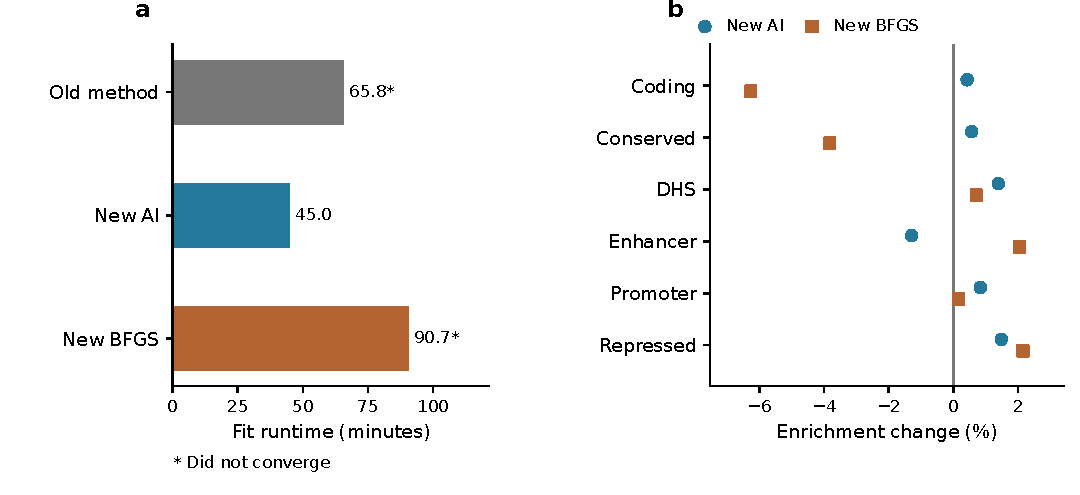
\includegraphics[width=\textwidth]{safeguarded_comparison/matched_optimizer_comparison.pdf}
\caption{Matched-start comparison for Weight with the penalty off; both integrated methods include the sufficient-progress safeguard. (a) Whole-process fitting time, excluding the separate historical endpoint audit. Asterisks identify fits that did not converge. (b) Relative changes in six marginal enrichment estimates compared with the historical endpoint; the vertical line denotes no change. AI passed the accurate local stationarity checks; historical and BFGS estimates remain provisional. Points are estimates without uncertainty intervals, and this comparison does not evaluate uncertainty calibration.}
\label{fig:matched}
\end{figure}

\begin{table}[H]
\centering\small
\begin{tabular}{lrr}
\toprule
Annotation & Old method & AI \\
\midrule
Coding & 8.249 & 8.284 \\
Conserved & 8.578 & 8.626 \\
DHS & 2.275 & 2.307 \\
Enhancer & 2.960 & 2.922 \\
Promoter & 3.034 & 3.059 \\
Repressed & 0.684 & 0.694 \\
\bottomrule
\end{tabular}

\caption{Marginal enrichment for the six main published categories in the matched-start Weight comparison. Historical and BFGS fits did not converge; AI passed the accurate local endpoint checks.}
\label{tab:matched}
\end{table}

\subsection{BFGS failure mechanism and safeguard evaluation}
Before the sufficient-progress safeguard was added, BFGS stopped after 76 iterations in 82.06 minutes with an exact-score line-search failure, $Q=4.593$, and likelihood 13.91 below the AI endpoint. This trajectory accepted its first trial at each of the first 74 iterations. It exhausted eight trials at iteration 75 and performed its first accurate-score refresh; the corresponding AI refreshes occurred at iterations 24 and 33. All eight trial gains following the BFGS refresh were numerically zero. Accurate-score correction therefore did not restore progress. Saved-array inspection identified extremely small absolute information for several saturated coefficients despite full rank after diagonal normalization. Such directions can produce enormous information-based proposals that cause the shared predictor cap to suppress changes in other coefficients. A fixed-endpoint diagnostic confirmed this mechanism: the reset-AI proposal was multiplied by $6.81\times10^{-20}$, leaving a predicted gain of $6.26\times10^{-19}$ below the numerical acceptance floor $1.49\times10^{-8}$. Its likelihood gain remained zero through 16 halvings. A scaled-gradient step improved the likelihood by 0.09930. Central directional differences agreed with its analytic directional derivative, and restoring the endpoint reproduced the parameters, likelihood, information and variant variances. The separate diagnostic took 9.72 minutes including loading, a precise derivative pass and 16 likelihood evaluations. A three-iteration native continuation using the safeguard then accepted two gradient steps, increasing likelihood by 0.184; it remained unconverged. This failure motivates further validation of the optimizer; it does not establish that BFGS updates are intrinsically inferior to AI.

The safeguarded BFGS fit from the same neutral start subsequently reached its 100-iteration cap in 90.66 minutes, with $Q=3.997$ and likelihood still 13.42 below the converged AI endpoint in the initial comparison. The first 74 objectives and accepted increments exactly matched the initial BFGS trajectory. After the accurate refresh, all 25 remaining steps used the gradient fallback and were accepted, but total likelihood improved by only 0.490 relative to the initial stalled BFGS endpoint. The sufficient-relative-gain trigger never activated. Thus the safeguard resolved the numerical zero-progress failure while leaving the poor optimization path largely unchanged. These results do not support selecting the tested BFGS variant as the default on performance grounds. AI with the same revised source converged and exactly reproduced the earlier parameters, heritability, enrichment, grouped derivatives and objective trajectory. All 31 proposal rows selected AI, with no fallback. Its unregularized uncertainty estimates closely agreed with the earlier well-behaved fit: maximum coefficient-standard-error difference was $5.6\times10^{-10}$. This checks numerical stability at this endpoint without establishing uncertainty calibration generally.

\subsection{BMI working-trait control}
BMI was selected because the earlier 97-annotation fit reported native convergence. From the same neutral start and using the same revised implementation, both AI and safeguarded BFGS passed the precise endpoint checks. AI required 26 iterations and 22 accepted steps, with $Q=0.0003844$; BFGS required 37 iterations and 34 accepted steps, with $Q=0.0004001$. The maximum signed objective gain for BFGS was 0.0003069, below the 0.001 tolerance; all four AI gains were negative. Process times were 39.18 minutes for AI and 45.39 minutes for BFGS, with optimizer times 36.79 and 42.99 minutes. AI used 27 full derivative passes including four precise passes; BFGS used 38 including three precise passes. Thus fewer precise audits did not give BFGS a runtime advantage on this trait.

Of BFGS's 35 proposal selections, 34 used BFGS and one used the AI reference. At iteration 5, the capped BFGS proposal's predicted gain was 58.26 versus 602.15 for AI, a ratio of 0.09676 below the prespecified 0.1 threshold. The accepted AI fallback increased the objective by 567.27. This confirms that the relative-gain safeguard can activate in a successful real-data fit; it does not isolate its causal effect on convergence or establish that 0.1 is optimal. AI's 23 proposals all retained AI. Each method had one exhausted line search followed by a precise refresh.

The final BFGS likelihood was lower than AI by 0.000180. Main enrichments differed by at most 0.061\% between the two integrated methods (Table~\ref{tab:bmicontrol}). The largest relative change across all 97 annotation summaries was for ExAC promoter flanks: 0.164238 under AI versus 0.158892 under BFGS ($-3.25$\%, absolute $-0.00535$). Total heritability was 0.266167 under AI and 0.266158 under BFGS. The two methods therefore reached similar objective values and primary estimates, with larger relative differences for one depleted secondary category.

\begin{table}[H]
\centering\small
\begin{tabular}{lrrr}
\toprule
Annotation & Prior native & New AI & New BFGS \\
\midrule
Coding & 7.039 & 7.006 & 7.008 \\
Conserved & 8.571 & 8.611 & 8.612 \\
DHS & 2.173 & 2.180 & 2.181 \\
Enhancer & 2.370 & 2.325 & 2.326 \\
Promoter & 2.489 & 2.492 & 2.491 \\
Repressed & 0.808 & 0.810 & 0.810 \\
\bottomrule
\end{tabular}

\caption{BMI marginal enrichment under the saved prior native fit and the two integrated optimizers. Both integrated fits passed precise stationarity checks. The prior fit reported convergence using likelihood-window stopping but failed the independent precise endpoint audit.}
\label{tab:bmicontrol}
\end{table}

The earlier BMI fit took 20.61 minutes and 16 iterations. Its likelihood was 0.7822 below the new AI fit; the largest main enrichment change was a 1.89\% decrease for enhancer regions. The earlier and integrated fits have different stopping rules and slightly different timer boundaries. These observed times document added cost on a previously successful trait but do not isolate a controlled implementation speed ratio. An independent audit reproduced the earlier endpoint likelihood exactly while retaining its saved parameters. It failed the stronger criteria: $Q=0.8057$ and a tested direction improved the likelihood by 0.7132, both above the 0.001 tolerance. Information remained full rank after diagonal normalization. The separate audit took 6.53 minutes and made no optimization updates. This confirms a convergence gap in the earlier result, without quantitatively attributing all added runtime to that gap. Taken together, the Weight and BMI comparisons do not support the tested BFGS variant as a performance default: it failed Weight and took longer than AI on BMI despite successful convergence there.

\subsection{Optional penalty: matched Weight and Hemoglobin comparisons}
Using the validated AI optimizer, we compared penalty weights zero and one from the same neutral start, with exact trial-penalty evaluation. The penalized fit passed the stationarity checks after 24 iterations and 21 accepted steps, with $Q=5.92\times10^{-5}$ and maximum signed objective gain $5.38\times10^{-6}$, below the $0.001$ tolerance. Its raw likelihood decreased by 0.876 relative to the unpenalized fit, as expected when maximizing a different objective. The final weighted global half-log-determinant was 149.2664. Total heritability increased from 0.287685 to 0.288064.

\begin{table}[H]
\centering\small
\begin{tabular}{lrrr}
\toprule
Annotation & Penalty off & Penalty on & Change (\%) \\
\midrule
Coding & 8.284 & 8.224 & -0.72 \\
Conserved & 8.626 & 8.528 & -1.14 \\
DHS & 2.307 & 2.302 & -0.22 \\
Enhancer & 2.922 & 2.917 & -0.16 \\
Promoter & 3.059 & 3.054 & -0.16 \\
Repressed & 0.694 & 0.694 & +0.05 \\
\bottomrule
\end{tabular}

\caption{Effect of the optional information penalty on the six main marginal enrichment estimates for Weight, using the same safeguarded AI implementation. Both fits passed the accurate penalized or unpenalized stationarity checks. Changes are relative to the penalty-off estimate. Uncertainty calibration is not evaluated.}
\label{tab:penaltyweight}
\end{table}

The largest change among the six primary enrichments was a 1.14\% decrease for conserved regions. All 97 fitted annotation summaries were retained for transparent assessment of secondary examples. Some model columns are signed continuous annotations, whose weighted summaries do not represent heritability fractions for sets of SNPs. The three secondary annotations displayed below were verified to contain only zero and one across all 22 source chromosome files, with no missing or nonfinite values; their source hashes match both fitted subsets.

The penalized fit took 38.09 minutes of subprocess time and 35.67 minutes in the optimizer, compared with 44.97 and 42.52 minutes without the penalty. The penalty changed the objective and optimization path, reducing iterations from 34 to 24, so these timings do not establish a general speed benefit. It used 25 full derivative passes, including three precise passes, 33 additional exact information evaluations taking 625.82 seconds, and 25 penalty-gradient contractions taking 31.48 seconds. All 21 proposal rows selected AI without fallback. Penalty uncertainty is evaluated using the retained approximation and its calibration remains untested.

For Hemoglobin, unpenalized AI passed the stationarity checks after 71 iterations and 67 accepted steps ($Q=0.0007232$). Penalized AI passed after 54 iterations and 51 accepted steps ($Q=0.0007072$), with maximum signed objective gain 0.0002811, below the 0.001 tolerance. All accepted proposals in both fits used AI. Total heritability increased from 0.193722 to 0.194172; raw likelihood decreased by 1.591, and the final penalty was 128.6598. The largest primary enrichment change was a 2.93\% increase for repressed regions (Table~\ref{tab:penaltyhemoglobin}).

\begin{table}[H]
\centering\small
\begin{tabular}{lrrr}
\toprule
Annotation & Penalty off & Penalty on & Change (\%) \\
\midrule
Coding & 11.652 & 11.436 & -1.86 \\
Conserved & 10.451 & 10.228 & -2.13 \\
DHS & 3.642 & 3.576 & -1.83 \\
Enhancer & 5.849 & 5.768 & -1.38 \\
Promoter & 3.989 & 3.965 & -0.59 \\
Repressed & 0.131 & 0.135 & +2.93 \\
\bottomrule
\end{tabular}

\caption{Effect of the optional information penalty on Hemoglobin's six primary marginal enrichments. Both AI fits passed the accurate endpoint checks. Changes are relative to the unpenalized estimate.}
\label{tab:penaltyhemoglobin}
\end{table}

Hemoglobin process times were 73.30 minutes without the penalty and 70.08 minutes with it; optimizer times were 70.92 and 67.68 minutes. Penalized optimization required 55 full derivative passes, including three precise passes, and 75 additional exact information evaluations taking 1,431.57 seconds. Its 55 penalty-gradient contractions took 69.00 seconds. These costs were offset by fewer iterations in this comparison; the findings do not establish that the penalty generally reduces runtime.

\begin{figure}[H]
\centering
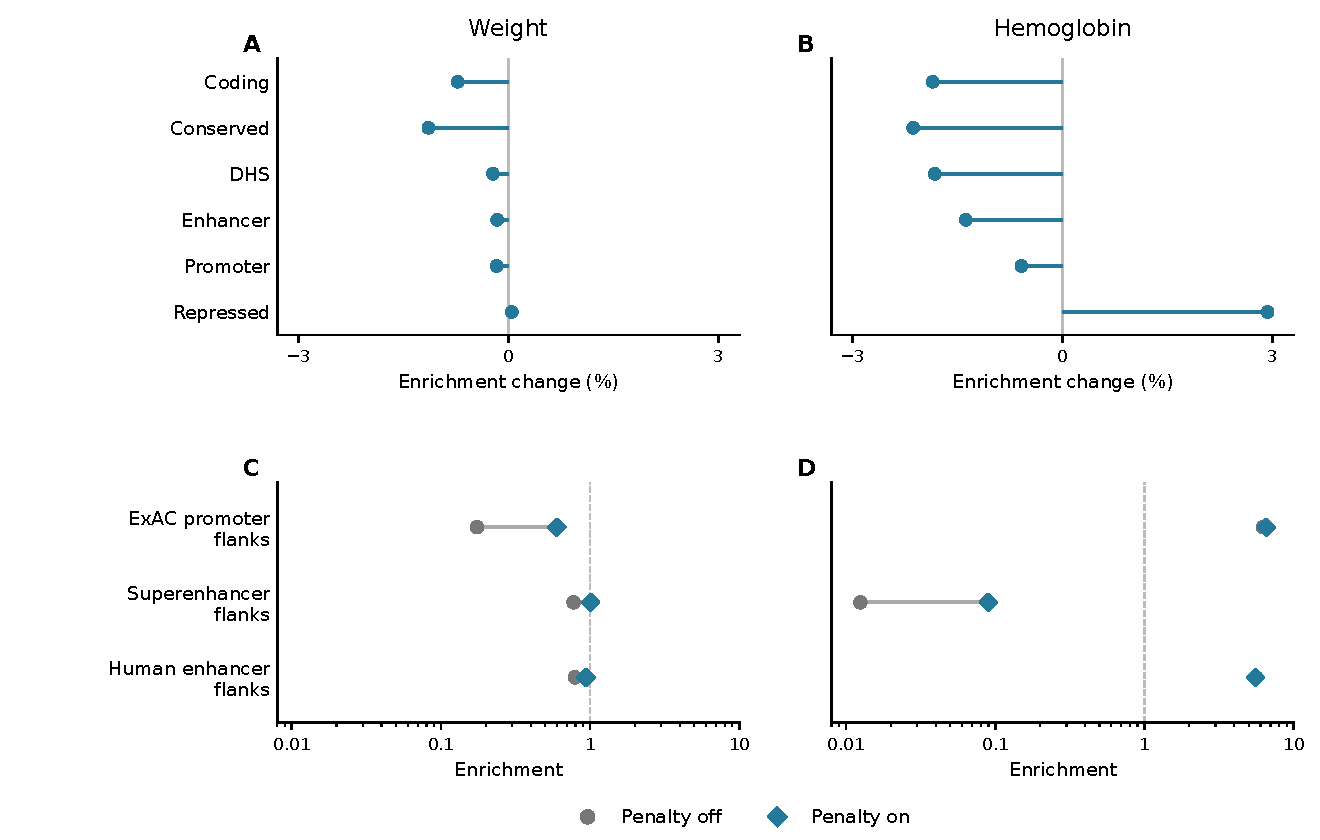
\includegraphics[width=\textwidth]{penalty_comparison/penalty_enrichment_comparison.pdf}
\caption{Information-penalty effects on marginal enrichment using AI. A--B, relative changes for the six annotations displayed in the published manuscript. C--D, unpenalized and penalized estimates for three binary flank annotations, on a logarithmic axis; the dashed line marks enrichment one. These secondary annotations were selected for large changes in Weight before the Hemoglobin penalty endpoint was obtained; all three are shown for both traits. All four fits passed the precise endpoint checks. The display concerns point estimates; uncertainty calibration is deferred.}
\label{fig:penalty}
\end{figure}

\begingroup\clubpenalty=10000
For Weight, ExAC promoter-flank enrichment increased from 0.1745 to 0.5994, superenhancer-flank enrichment from 0.7757 to 1.0117, and human-enhancer-flank enrichment from 0.7926 to 0.9378 (Figure~\ref{fig:penalty}). For Hemoglobin, superenhancer-flank enrichment increased from 0.01247 to 0.08976: a large relative increase of 620\%, but an absolute increase of 0.0773, with substantial depletion remaining. The other two secondary categories changed by +5.22\% and $-0.62$\%, respectively. The analyzed sets contain 4,417 ExAC promoter-flank SNPs and 22,510 superenhancer-flank SNPs in each trait; human-enhancer flanks contain 70,070 SNPs for Weight and 70,074 for Hemoglobin. These marginal summaries account for overlapping annotations. Changes in an individual coefficient do not directly measure changes in a category's marginal heritability.\par\endgroup

Counterfactual screening diagnostics identified eight trials in the exact Weight fit that a linear penalty screen would reject, including two accepted by the exact procedure. In Hemoglobin, the corresponding counts were 37 and 19. These observations demonstrate a false-rejection risk; they do not measure the behavior or speed of the implemented screening-and-fallback procedure, which can change the subsequent path. The completed matched Weight comparison found no runtime benefit from screening (Table~\ref{tab:screenmatched}). Both strategies passed the precise stationarity checks in 24 native iterations. The screened fit accepted 20 steps versus 21 for exact evaluation, ending with $Q=9.93\times10^{-5}$ and a penalized objective lower by $6.29\times10^{-5}$. Screening saved five trial-information evaluations but added 25 likelihood-only evaluations and one precise audit. Optimizer time increased by 6.46\%. This comparison supports retaining exact trial evaluation as the default.

\begin{table}[H]
\centering\small
\begin{tabular}{lrr}
\toprule
Measure & Exact & Linear screen \\
\midrule
Process time (min) & 38.09 & 40.37 \\
Optimizer time (min) & 35.67 & 37.98 \\
Iterations & 24 & 24 \\
Accepted steps & 21 & 20 \\
Full derivative passes & 25 & 25 \\
Precise passes (included above) & 3 & 4 \\
Trial-information evaluations & 33 & 28 \\
Likelihood-only evaluations & 0 & 25 \\
\bottomrule
\end{tabular}

\caption{Exact versus linear-screen trial evaluation for the matched penalized Weight fit. Both strategies use the same AI implementation and starting point. Precise passes are included in the full-pass count. Timings include the final precise calculation.}
\label{tab:screenmatched}
\end{table}

Six proposals were screened out, and one line search invoked the exact fallback. The within-run counter recorded no rescued previously screened accepted steps. This does not imply that screening caused no false rejections: the paired runs have identical recorded accepted trials, proposals and objectives through iteration 18. At iteration 19 the screen skipped a full step that the exact run accepted with objective gain 0.002519, then accepted a half step with gain 0.036403. Thus screening changed the trajectory even though the exact-fallback counter did not identify this event.

The largest relative difference among the six primary enrichments was 0.00677\%. Across all 97 annotation summaries, ExAC promoter-flank enrichment changed most, from 0.599381 under exact evaluation to 0.608331 under screening (+1.49\%, absolute +0.00895). Total heritability differed by $-1.67\times10^{-6}$. These differences illustrate that close objective values and passed local stopping checks can coexist with larger relative changes in a depleted category. They do not establish equivalence of parameter estimates or uncertainty calibration.

\section{Stopping criteria and interpretation}
For an interior point with positive-definite information, define the undamped information-scaled score criterion
\begin{equation}
 Q(\theta)=\frac12g(\theta)^\mathsf{T}I(\theta)^{-1}g(\theta).
 \label{eq:stop}
\end{equation}
It is the predicted improvement of the information-based quadratic model, not a bound on the actual remaining likelihood gain. Small damped updates, small successive objective increments, or small fixed-probe scores trigger further checking rather than establish stationarity.

The integrated procedure requires a fresh accurate score at the returned parameters and $Q\leq10^{-3}$. It also evaluates actual objective changes in both signs of the limited information-scoring direction and a scaled gradient direction, requiring none to improve the objective by more than $10^{-3}$. Positive definiteness is checked separately on diagonally normalized information. These finite directional checks provide additional local evidence; neither they nor equation~\eqref{eq:stop} establish global optimality. Distinct starting points remain necessary to assess alternative stationary endpoints. With the penalty enabled, these checks use $g_w$ and $F_w$; their operating characteristics remain to be evaluated. The default iteration cap is 100, and the default criterion is $10^{-3}$. This tolerance measures local stationarity; the historical implementation instead applied its tolerance to successive likelihood increments.

For low-dimensional models, an experimental audit estimates blockwise central finite-difference scores at two perturbation sizes. It checks both their disagreement and a floating-point resolution diagnostic, falling back to analytic accurate scores if the diagnostic fails. This is an empirical accuracy check rather than a rigorous error bound. The integrated implementation uses accurate inverse diagonals for all model sizes. Their cost motivates selective audits.

When an unpenalized variance approaches zero, the link Jacobian can vanish and ordinary coefficient-space criteria can behave poorly. Analysis-specific profiles and one-sided variance perturbations help explain such endpoints. They are \emph{diagnostics only}: they do not form a boundary-acceptance feature of the proposed optimizer and do not count as validation of the general procedure. Penalized fits are evaluated directly on equation~\eqref{eq:penalty}. Whether regularization resolves the observed saturated fits is an empirical question.

\section{Numerical consistency and uncertainty}
Every trial evaluation must correspond to its stated parameters. To avoid cancellation after extreme proposals, the worker reconstructs covariance diagonals from the fixed residual diagonal and the current aggregated genetic variance in equation~\eqref{eq:cov}. Rejected trials restore the accepted state; invalid trial values cannot be accepted. Final scores and information are refreshed at returned parameters. These safeguards prevent changes in the numerical state from masquerading as changes in the statistical objective.

At a fixed covariance, inverse-diagonal probe solves can reuse the current sparse Cholesky factor. The historical analysis runner already provided a validated guarded override for this reuse; the historical comparator retains that execution optimization, while the integrated package supplies it directly. This shared setting avoids comparing BFGS with an unnecessarily slow iterative probe implementation. Accurate inverse diagonals in the integrated methods are calculated by triangular inversion of the Cholesky factor: in factorization order, the diagonal entries are the squared column norms of $L^{-1}$, with the permutation subsequently undone. These exact audits still require dense triangular workspace and are used selectively. Both integrated AI and BFGS share the accurate-audit implementation; their comparison isolates proposal-metric choice more closely.

For unpenalized one-step delete-group reconstruction, if $g_{-r}$ and $I_{-r}$ are the retained-data score and positive information evaluated at the full-data fit, the Newton approximation has sign
\begin{equation}
 \widehat\theta_{-r}\simeq\widehat\theta+I_{-r}^{-1}g_{-r}.
\end{equation}
The implementation corrects the update sign and evaluates derivatives at the returned fit. The inferential solve now uses symmetric diagonal scaling and Cholesky factorization without an absolute ridge. Writing $D_{jj}=\sqrt{(I_{-r})_{jj}}$ and $C=D^{-1}I_{-r}D^{-1}$, the update is $D^{-1}C^{-1}D^{-1}g_{-r}$. Positive definiteness and numerical rank are checked on $C$; invalid solves produce unavailable uncertainty. This preserves the calculation under changes of coefficient units. A fixed positive ridge previously added to the negative Hessian overwhelmed curvature in saturated directions and could produce artificially small standard errors. The initial frozen fits retain those provisional outputs; the figures here compare point estimates only. Focused regression tests cover the tiny-curvature sign error and coordinate rescaling. This numerical repair does not evaluate the statistical validity of a local approximation far from a stationary endpoint. Agreement of a reconstructed update with this formula verifies implementation, not uncertainty calibration. For penalized fits, delete-group reconstruction uses likelihood scores and information at the penalized endpoint, with explicit metadata identifying this approximation. Penalized objective gradients are reported separately. Singular information produces unavailable uncertainty, and unresolved endpoints are labelled provisional. Calibration, penalty curvature in uncertainty calculations, and penalized delete-group inference remain deferred.

\begin{thebibliography}{9}
\bibitem{gilmour} Gilmour, A. R. (2019). Average information residual maximum likelihood in practice. \emph{Journal of Animal Breeding and Genetics}, 136, 262--272. \href{https://doi.org/10.1111/jbg.12398}{doi:10.1111/jbg.12398}.
\bibitem{firth} Firth, D. (1993). Bias reduction of maximum likelihood estimates. \emph{Biometrika}, 80, 27--38. \href{https://doi.org/10.1093/biomet/80.1.27}{doi:10.1093/biomet/80.1.27}.
\bibitem{li} Li, H., Kamath, T., Mazumder, R., Lin, X., and O'Connor, L. J. (2026). Improved heritability partitioning and enrichment analyses using summary statistics with graphREML. \emph{Nature Genetics}, 58, 1573--1582. \href{https://doi.org/10.1038/s41588-026-02649-0}{doi:10.1038/s41588-026-02649-0}.
\end{thebibliography}
\end{document}
